\section{Error Confinement in JPEG Application} \label{sec:jpeg}

JPEG is a commonly used lossy compression technique of digital images, which offers selectable compression degree to trade off between storage size and image quality. JPEG consists of several major steps including color space transformation and down sampling. In this work, we focus on the subsystem shown in Figure \ref{fig:qos_jpeg} which consists of four major blocks, the 2D Discrete Cosine Transformation (2-D DCT), Quantization, De-quantization and 2D Inverse Discrete Cosine Transformation (2-D IDCT). Figure \ref{fig:qos_jpeg} also shows the different stages of the processing image as it propagates through the system. The quality of the output image is evaluated using PSNR \cite{huynh2008scope}. A typical PSNR value for lossy image is 30 dB. The final output image in Figure \ref{fig:qos_jpeg} has a PSNR of 39.22 dB, which is intrinsic tolerable due to the perceptual limitations of human brain.

\paragraph{2-D DCT} is widely adopted in digital image and video processing. It transfers individual $8 \times 8$ image block from spatial domain to frequency domain. The conventional DCT principle could be referred in \cite{gonzalez2009digital} while there exists low power and fault tolerant implementation for 2-D DCT \cite{august2004low}\cite{banerjee2007process}. The output $8 \times 8$ matrix of DCT contains the frequency coefficients which affect the image quality. However, their impacts are non-uniform. According to \cite{banerjee2007process} the first 20 coefficients control 85\% of the input image quality while the rest 44 coefficients have significantly less contribution in improving the image quality. 2-D IDCT is the inverse operation of DCT, which transforms the coefficient in frequency domain back to the spatial domain.

\paragraph{Quantization} is used to compress the image according to different JPEG standard. Each element in the input matrix is divided by a coefficient in the quantization matrix. This usually leads to a matrix with non-zero numbers on the top-left corner while zeros in other part of the matrix. De-quantization is the inverse operation of quantization, which scales up the value by multiply the same coefficient in the quantization matrix.

\begin{figure}
\centering
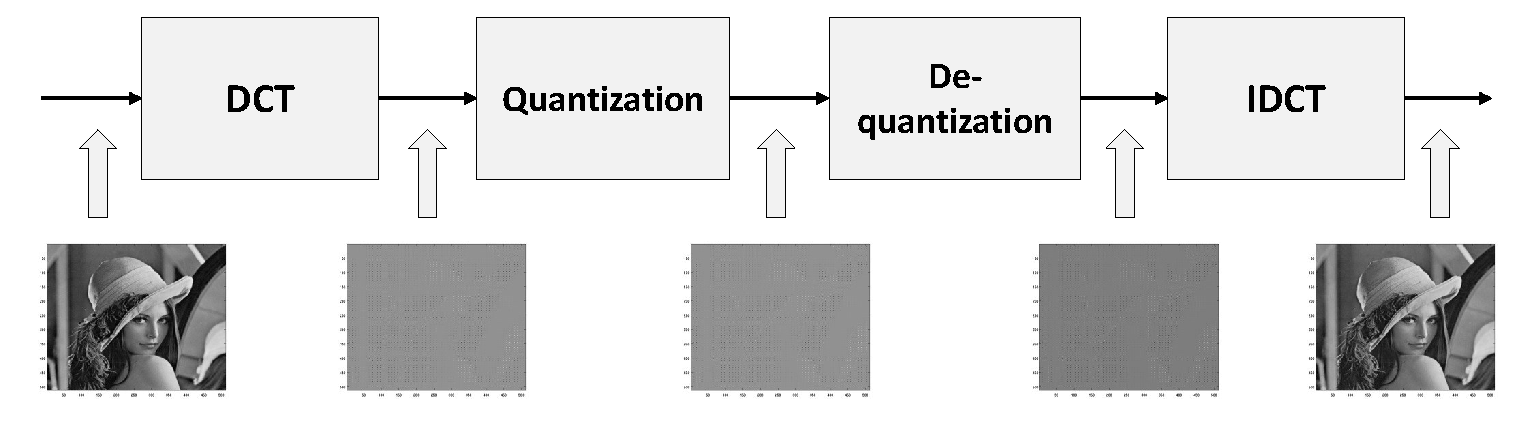
\includegraphics[width=90mm]{./eps/qos_jpeg}
\caption{Subsystem in JPEG application}
\vspace{-3mm}
\label{fig:qos_jpeg}
\end{figure}
%\vspace{-5mm}

The input image which has the resolution of $512 \times 512$ is decomposed into 4,096 matrices of the size $8 \times 8$, where each matrix is being processed individually. Simulation shows that the individual output matrix shares similar pattern, where the top-left corner of both DCT and quantization output matrix exhibits larger number, while the rest ones remains small and even zero for quantization output matrix. Figure \ref{fig:qos_matrix} shows the element wise average matrix for the complete 4,096 individual matrix, which are adopted as the reference matrix for error confinement.

\begin{figure}
\centering
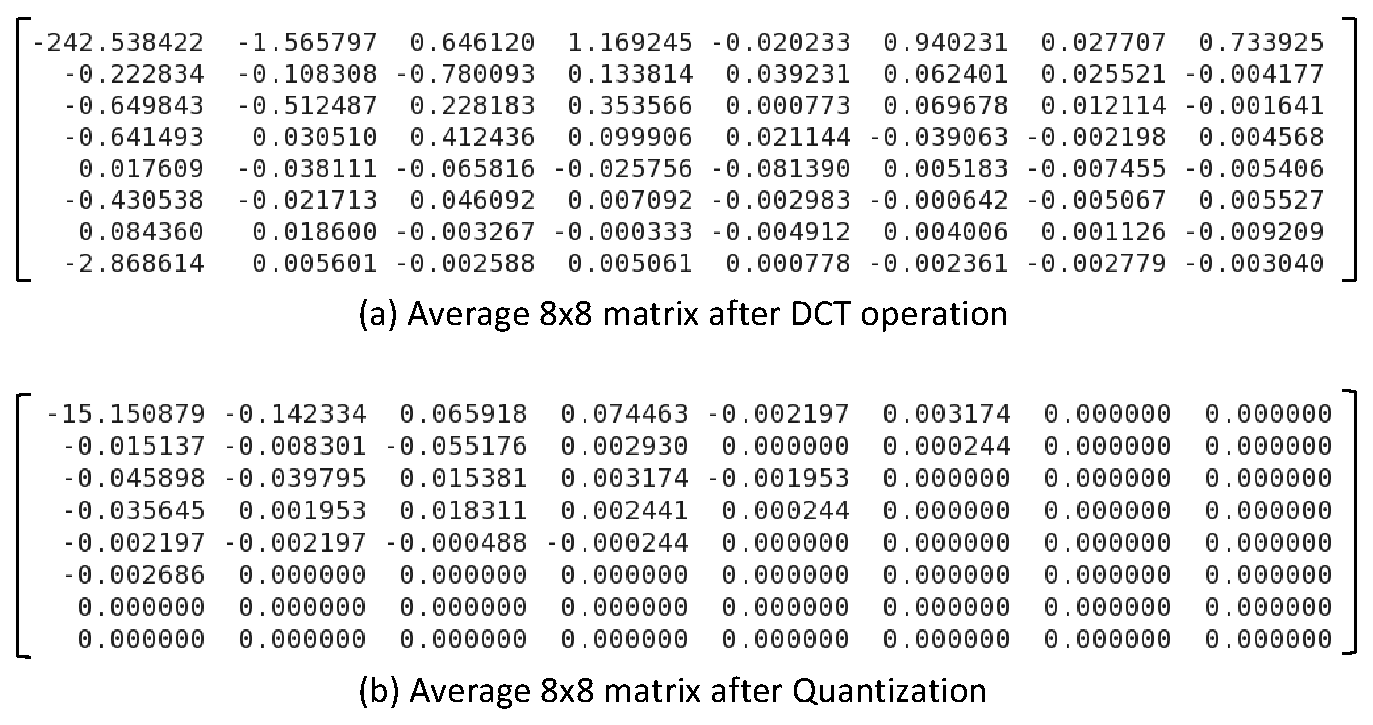
\includegraphics[width=80mm]{./eps/qos_matrix}
\caption{Error confinement matrix for DCT and Quantization Coefficients}
\vspace{-3mm}
\label{fig:qos_matrix}
\end{figure}
%\vspace{-5mm}

